\documentclass[12pt]{article}
\usepackage{graphicx, subfigure, float, amsmath, amssymb}
\usepackage[margin = 1.0 in]{geometry}
%\usepackage[style = nature]{biblatex}
\title{Comparing Site Variability Among Natural and Designed Proteins}
\author{Eleisha Jackson \and Art Covert \and Noah Ollikainen \and Tanja Kortemme \and Claus Wilke}
\begin{document}

\date{\today}
\maketitle

%Use \textbf{} to bold tetxt
\section{Abstract}
\label{Abstract}
Protein structure prediction software attempts to create protein structures that are structurally similar to natural proteins. We examine how accurately Rosetta, a protein prediction software, reconstructs observed patterns of variability found in natural proteins. We use Rosetta to design proteins and then compare these designed proteins with natural proteins. Our comparisons include site variability, observed distributions at sites and the effects of protein structure on site variability. Proteins designed with a fixed backbone underestimate the amount of site variability observed in natural proteins while proteins designed with a flexible backbone result in more site variability. Intermediate flexibility during design results in site variability patterns that most accurately resemble those found in natural proteins. From these results we conclude that intermediate backbone flexibility during design results in more accurate protein design and that scoring functions that determine acceptable substitutions must improve to account for structural constraints on site variability patterns.

\section{Introduction}
\label{Introduction}

There are many selective pressures that affect the rate at which protein sequences change over time. Some of these important determinants include protein dispensability, expression and protein structure. A protein's structure determines how it can function and interact with other proteins.  Therefore a thorough knowledge of the constraints of protein structure on protein evolution is necessary to understand how proteins function. Many proteins need stable native structure to preserve their function. Understanding how proteins function and evolve is of critical importance for the development of proteins with novel functions, advances in drug therapy and increasing our knowledge of disease.  

\par It is well documented that protein structure has an influence on variability seen at sites \cite{Franzosa2009, Ramsey2011}. Computational protein design can be used develop and analyze protein structures allowing us to further our knowledge of the effects of protein structure on sequence evolution. In fact recent work using knowledge gained from computational design has resulted in the design of proteins that bind to an influenza virus \cite{Fleishman2011}. During design, protein sequences are optimized for stability \cite{Butterfoss2006, Das2008}. Protein stability has been shown to be an important selective force on proteins \cite{Drummond2008}. Therefore these optimized structures can be used to assess the constraints of structural stability on protein sequences. Comparing designed and natural proteins will allow us to understand how protein structure, and in particular, protein stability shape observed sequence patterns.

\par In this paper, we assess the ability of designed proteins to re-capture natural sequence properties by directly measuring variability patterns and comparing them to observed patterns in natural proteins. We not only examine how similar site variability is but we also examine whether the relationships between site position and variability in natural proteins are maintained in designed proteins.  First we obtained a selection of natural proteins and used the design software, Rosetta (http://www.rosettacommons.org/), to design proteins that are structurally similar. We then measured site variability within the natural proteins and compared this variability to the variability within the designed proteins. We also compared the amino acid distributions at sites within natural proteins with that of sites in designed proteins. Lastly we compared how structure constrains sequence variability within both types of proteins (natural and designed). By directly measuring and comparing amino acid patterns of designed proteins with natural proteins, we can determine which properties in natural proteins designed proteins accurately capture. 

\section{Methods}
\label{Methods}

\par In order to begin our comparison, we analyzed two separate protein datasets. For first dataset, we obtained 38 Saccharomyces (yeast) proteins from the Protein Database (PDB).  For each protein, we acquired a series of homologous sequences from the dataset Ref. \cite{Ramsey2011}. These homologous sequences were found using BLAST against the Saccharomyces Genome Database (SGD) as described \cite{Ramsey2011}. These sequences were aligned with the protein alignment software MAFFT \cite{Katoh2002}. Our resulting dataset was comprised of 38 natural sequence alignments with at least 50 sequences. We created similar designed protein alignments using the protein design software Rosetta. Each of the 38 natural proteins was used to design a series of proteins that are structurally similar to the natural protein structure.

\par During the design process we allowed for a fixed backbone and a flexible backbone. In the fixed design, the backbone of the amino acids was fixed and only the side chains were allowed to move. In other designs, we allowed the backbone itself to move. For the flexible backbone designs we used Backrub, a package in Rosetta \cite{Smith2008}. In Backrub, we used a temperature parameter that controlled how flexible the backbone was allowed to be during design. A temperature of zero corresponded to a fixed backbone scenario and by increasing the temperature we allowed the backbone to be more flexible. The parameters used for the flexible backbone design were 0.03, 0.1, 0.3, 0.6, 0.9, and 1.2. 
\par Our second dataset was comprised of protein domains. We obtained 40 protein domains for which there were crystal structures in the PDB representing these protein domains.  We created protein alignments for each protein structure by acquiring homologous sequences for each protein from the Pfam database (insert citation) and aligning the sequences as detailed in Ref. (reference their paper?).   For each of the the 40 protein domains a series of 500 proteins  were designed using the protein domain as a template. For these proteins, in addition to a fixed backbone design treatment, protein domains were designed with Backrub using temperatures of 0.3, 0.6, 0.9, 1.2, 1.8, and 2.4. Protein domain sequences were also designed for fixed backbones using an alternative method. In this method the energy function used during sequence design dampens the weight of the repulsive Lennard-Jones (LJ) potential term. We call this method "Soft".  We used MUSCLE \cite{Edgar2004} to align our designed sequences. The result was a series of designed protein alignments of 500 sequences for each original natural protein at various temperatures.  We performed our analysis on two independent sets to verify that our results were not a result of the inherent sequence variation between the specific protein sequences in the dataset used for the analysis. 
\par In order to assess the quality of the designed sequences we compared the natural sequence alignments to the designed sequence alignments. Our metrics of comparison included site variability, amino acid distribution similarity at sites, and structural design accuracy. The variability of a site was quantified by calculating the entropy of the site amino acid distribution of that site in an alignment. 
The entropy (H) of an amino acid distribution is	$$ \sum_{i=0}^{n}p_iln{\left(p_i \right)} $$

where n is 20, the number of canonical amino acids, and $p(i)$ is the frequency of an amino acid at that site. 
We quantified the shape of an amino acid distribution at a site with the Kullback - Leibler Divergence (KL Divergence). 
The KL Divergence for a site is given by
	$$ \sum_{i=0}^nln  \left({\frac{p(i)}{Q(i)}}\right) P\left(i\right) $$
$P(i)$ is the frequency of an amino acid at a given site in a natural protein. $Q(i)$ is the frequency of that amino acid at the same site within the designed protein that is being compared.
In order to observe how structure influence observed amino acid patterns we used Relative Solvent Accessibility (RSA) at sites. We calculated the Solvent Accessibility (SA) of sites using the software DSSP \cite{Kabsch1983}. We normalized the SA values by using the values in Ref. \cite{Tien} and obtained the appropriate Relative Solvent Accessibility values for each site. 

\section{Results}
\label{Results}

\subsection{Site Variability}
\label{SiteVariability}
%Figure 1
\begin{figure}[H]
%\centering
\centerline{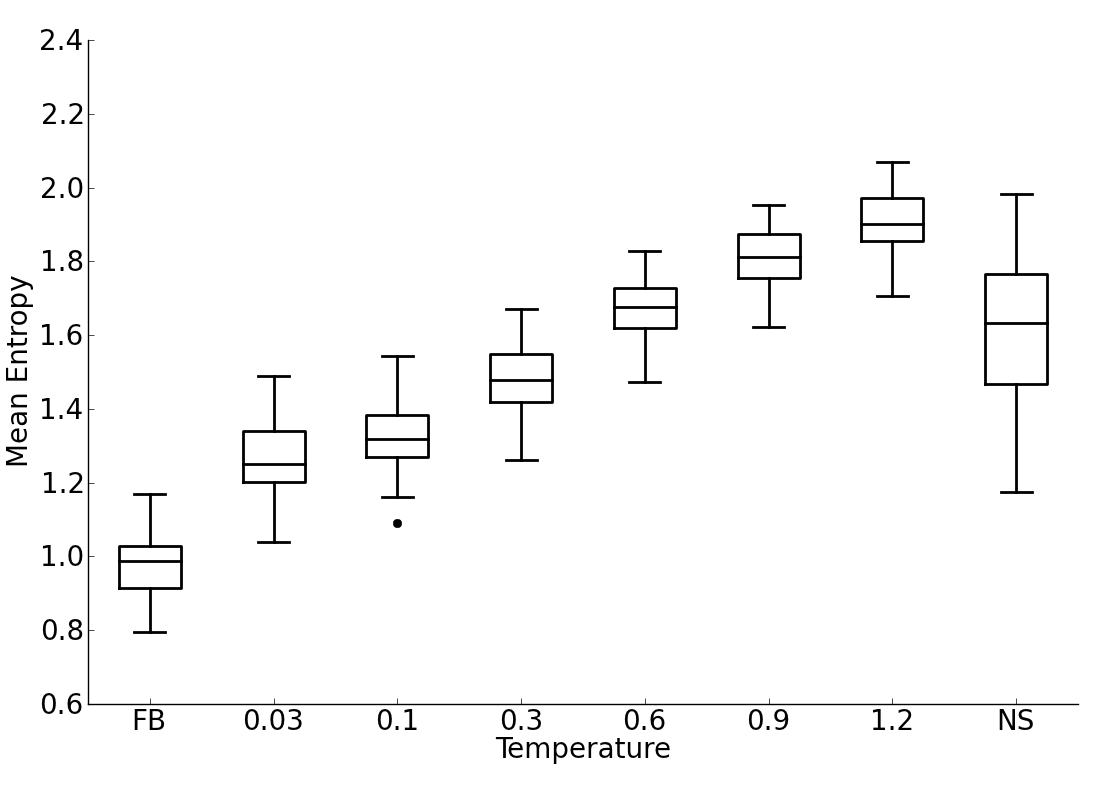
\includegraphics[width = 6in]{figures/Mean_Entropy_vs_Temp_Boxplot.png}}
\caption{Mean Entropy versus temperature for a series of proteins. Each designed protein was created using one of 38 proteins as template. The temperature refers to the temperature used during the design process. Higher temperatures allowed for more backbone flexibility. FB and NS refer to the fixed backbone designed proteins and natural proteins respectively.  As the backbone becomes more flexible during design, sites exhibit increased variability.}
\label{SiteVarFig1}
\end{figure}

%Figure 13
\begin{figure}[H]
%\centering
\centerline{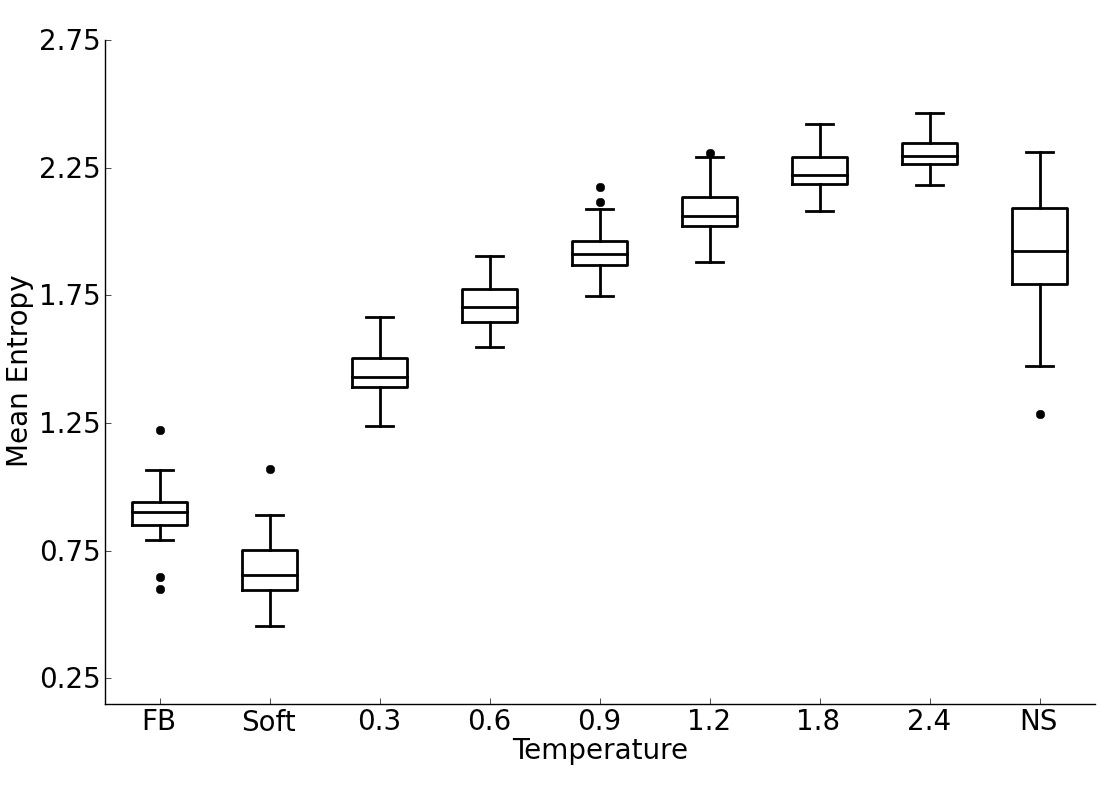
\includegraphics[width = 6in]{figures/Mean_Entropy_vs_Temp_Boxplot_Noah.png}}
\caption{Mean Entropy versus temperature for a series of designed proteins. The temperature refers to the temperature used during the designed process. Higher temperatures allowed for more backbone flexibility. FB and NS refer to the fixed backbone designed proteins and natural proteins respectively. Soft is an alternative method of fixed backbone design with a with a modified energy function.}
\label{NoahSiteVarFig1}
\end{figure}

%Figure 2
\begin{figure}[H]
\centering
\centerline{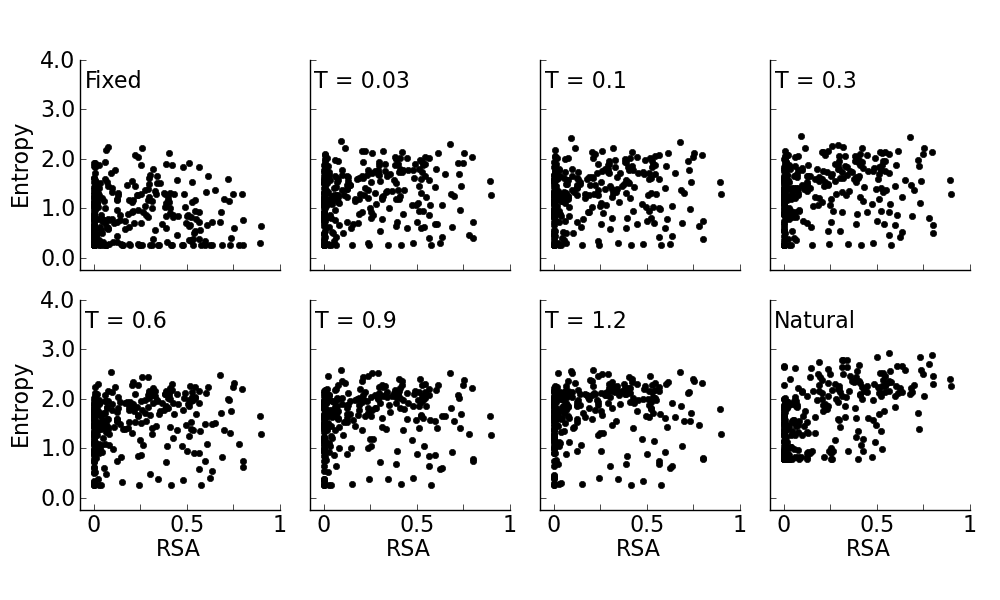
\includegraphics[width = 6.5in]{figures/RSA_vs_Entropy_1PV1_Combination_Plot.png}}
\caption{Entropy vs Relative Solvent Accessibility (RSA) for sites within the protein S - formylglutathione hydrolase (PDB: 1PV1, chain A). All RSA values are calculated from natural proteins. For most sites within the alignments created from the fixed backbone the entropy values are lower than they are in the natural proteins.  For designed proteins sites with backbone flexibility usually underestimate or overestimate entropy.}
\label{SiteVarFig2}
\end{figure}

\par Our goal was to understand how effective designed proteins were in recapturing the site variability in natural proteins. Therefore we compared the site variability in natural proteins with variability in the designed proteins as quantified by entropy.  We calculated the entropy for all sites in the natural and designed proteins. When using the fixed backbone approach to design proteins, the majority of sites were less variable in the designed proteins as opposed site variability seen in the natural proteins (Figure \ref{SiteVarFig1}). As the backbone became more flexible during the design process overall site variability increased. In fact, for most proteins there were a number of sites that overestimated site variability at that site when temperatures were high (Figures \ref{SiteVarFig2}, \ref{Entropy_Sites_Noah}). Intermediate temperatures appeared to be the best at estimating site variability suggesting that proteins designed at these temperatures with moderate backbone flexibility are more effective at approximating natural site variability (Figures \ref{SiteVarFig1}, \ref{Mean_Entropy_Noah}). Proteins designed with a temperature of 0.6 and 0.9 had site variability that mostly closely resembled site variability in natural proteins.
 \par In order to examine whether there was a difference in the mean entropy of sites in the core of the protein and those on the surface we calculated the mean entropy for sites according to how buried they were. Sites were classified as either buried, partially buried, and or exposed if they had an RSA value of less than 0.05, a value between 0.05 and 0.25 inclusive, and a value greater than 0.25 respectively. Both buried and partially buried sites exhibited trends similar to those observed when you compare the mean values of all sites. For example, for buried residues within the first dataset of 38 whole proteins, a temperature of 0.6 is optimal. However, within these same proteins, surface sites have a optimal temperature of 0.9 (Figure \ref{Duncan_Position_Entropy}). Therefore in order to capture the site variability that is seen at surface sites, one has to design proteins with a more flexible backbone compared to that used for buried sites if you want to recover the site variability seen in natural proteins. The amount of site variability tells us nothing about whether the types of amino acids found at each site were similar. For insight we investigated the amino acid distributions at sites within the two types of proteins for similarities and dissimilarities. 

\subsection{Assessing Similarity of Amino Acid Distributions}
\label{AminoAcidDistributions}

\par Next we assessed the amino acid distributions of the designed sequence alignments and compared the similarity to the natural sequence alignments. The Kullback-Leibler (KL) Divergence for a site measures how similar the amino acid distribution of a site is to the same site in the natural protein that was used in the design process. A KL Divergence value of zero implies that the distributions are exact. The higher the KL Divergence Value, the more dissimilar two distributions are.  We also calculated the mean KL Divergence across sites per protein to find, on average, how accurately the amino acid distributions in the designed proteins distributions of the natural proteins.  In order to have a basis of comparison for how well proteins approximate themselves we also calculated the mean KL Divergence of natural proteins. We calculated the KL Divergence value of natural sites in the natural alignments by splitting the alignments in half. One half was used as the true distribution and the other was used as the simulated distribution. This allowed us to calculate how effective the natural proteins are at predicting their own distributions. Performing this comparison allows us to quantify how accurately Rosetta designs proteins that have the proper amino acid distributions at sites and for which temperatures it is more effective at capturing the proper amino acid distribution seen in natural protein alignments. 
\par Through our analysis we found that as temperature increases, the mean KL Divergence value decreases (Figure \ref{AADisFig1}A). This corresponds to the distributions at sites within these proteins being more similar to those in the natural proteins. In addition, higher temperatures were better at simulating the proper distributions  at sites. However, this can be misleading. As mentioned earlier, as the temperature was increased during design, the backbone was more flexible. This allows for more substitutions within the protein causing the amino acid distribution to be more uniform. By chance this might result in the designed site distributions overlapping with the natural distributions and appearing to capture more of the natural distributions. 

%Figure 12
\begin{figure}[H]
%\centering
\centerline{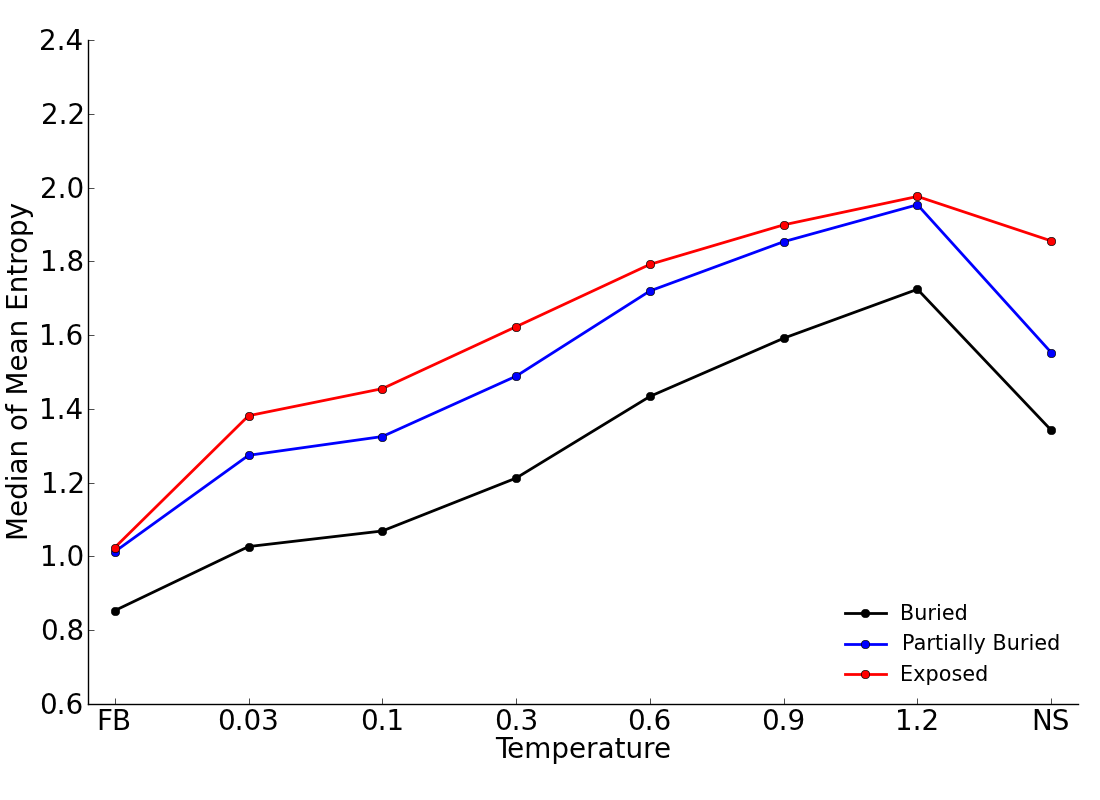
\includegraphics[width = 6in]{figures/Mean_Entropy_Position_Lineplot.png}}
\caption{Median of Mean Entropy versus Temperature sites within series of designed proteins.  Sites are classified as buried, partially buried, or exposed based on RSA magnitude. The temperature refers to the temperature used during the designed process. Higher temperatures allowed for more backbone flexibility. FB and NS refer to the fixed backbone designed proteins and natural proteins respectively.}
\label{Duncan_Position_Entropy}
\end{figure}
 

%Figure 3
\begin{figure}[H]
\centerline{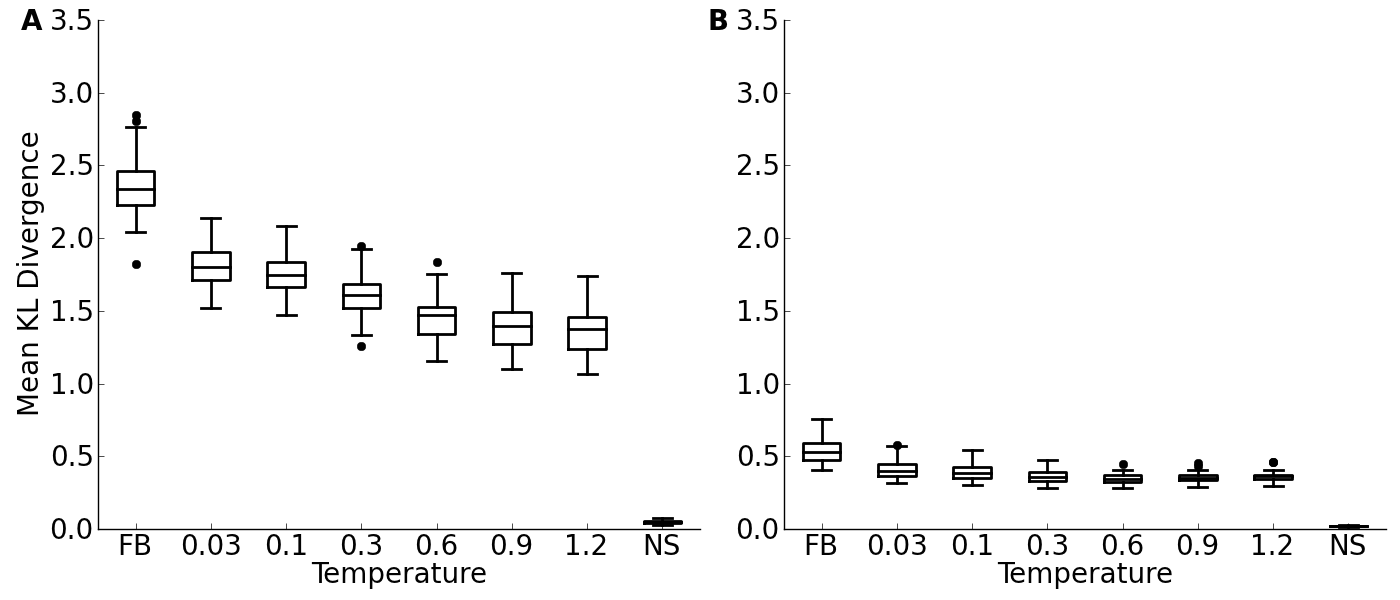
\includegraphics[width = 6in]{figures/Mean_KL_vs_Temp_Boxplot.png}}
\caption{Mean Kullback-Leibler (KL) Divergence Value vs Protein Design Temperature. Each boxplot corresponds to the mean KL Value for each of 500 designed proteins. Higher KL Divergence  equals a less similar distribution. The temperature refers to the temperature used when designing the proteins using BACKRUB and Mean KL Divergence stands for the mean Kullback-Liebler Divergence for each protein.  A) For these distributions, the amino acids are ordered by amino acid type, e.g., alanine, tyrosine. B) For these distributions the amino acids are ranked and ordered by their frequency with more frequent amino acids ranked first. Higher temperatures result in more backbone flexibility during design. Proteins designed with a fixed backbone have a less similar amino acid distribution than designed proteins with flexible backbones.}
\label{AADisFig1}
\end{figure}

\par To further explore this observation we ordered amino acids by frequency. After this ordering process we observed that the trend between backbone flexibility and KL Divergence did not hold. Notice KL Divergence decreases as temperatures rose into the intermediate range (i.e., 0.3, 0.6), and increased slightly as temperature increased past that point (Figure \ref{AADisFig1}B). Since the amino acids are ordered by frequency, we know any similarity is not just a result of a flatter, more spread out distribution. This suggests that intermediate temperatures are better at capturing the behavior and shape of the natural distributions. Consequently, when designing proteins using Rosetta, intermediate temperatures that result in moderate backbone flexibility result in proteins that have more similar amino acid distribution to those found in natural proteins. These trends that we observed all apply to all sites with a site regardless of whether a site was classified as buried, partially buried, or exposed. This was the case for both datasets we analyzed.  Up until this point, we have focused sequence similarity. However, Rosetta is a structure design software. Therefore, in addition to examining the sequence behavior we also examined how the Rosetta addressed the constraints imposed by structure on sites. 

\subsection{How does protein structure determine design accuracy?}
\label{ProteinStructure}

%Figure 4
\begin{figure}[H]
\centering
\centerline{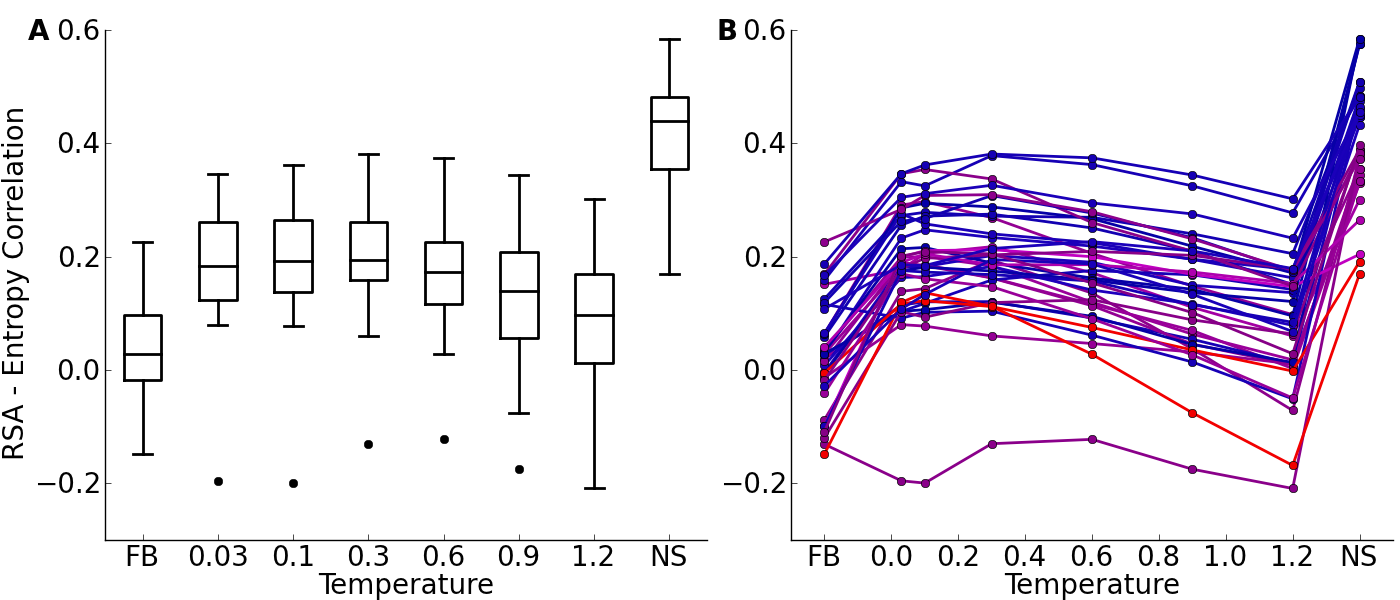
\includegraphics[width = 6in]{figures/Cor_Mean_Entropy_RSA_Combination_Plot.png}}
\caption{Correlation between Entropy and RSA for sites within proteins.  The temperatures represent alignments of designed proteins where an increased temperature relates to an increase level of backbone flexibility during the design process. A) Boxplots of the correlation between RSA and site entropy for various protein alignments. B) Lineplots of the correlation between RSA and site entropy for various protein alignments. The colors correspond to the value of the strength of the correlation between entropy and RSA at sites. Natural proteins have a higher correlation between RSA and entropy at sites.}
\label{StructureFig1}
\end{figure}

\par We wanted to determine how protein structure constrains protein sequence variability using Rosetta. In particular we were interested in how closely the designed proteins captured the relationship between structure and sequence variability within natural proteins. The Relative Solvent Accessibility (RSA) of a site quantifies how buried a residue is within the protein's core \cite{Franzosa2009}.  A lower RSA value means a residue is more buried. By correlating the RSA value of a site with its entropy we can examine the relationship between structure and site variability (as measured by entropy).  On average within the natural proteins there was a higher correlation between entropy and RSA at sites (Figure \ref{StructureFig1}A, \ref{NoahStructureFig1}A) as compared to the designed. This means that sites on the surface of a protein experience greater site variability compared to sites within the protein's core. In addition, proteins with a higher correlation between RSA and entropy in the natural proteins have a higher correlation in the designed proteins (Figure \ref{StructureFig1}B, \ref{NoahStructureFig1}B). However, designed proteins did not perfectly capture the relationship between structure and site variability. 

\par Overall the designed proteins have a lower correlation between RSA and entropy.  In general, the fixed backbone treatment resulted in a lower correlation between entropy and RSA at sites suggesting there were not enough substitutions made on the surface.  This applied to both fixed backbone methods. Among the designed proteins, intermediate temperatures had a higher correlation between entropy and RSA at sites. For example in the dataset comprised of 40 proteins, temperatures of 0.03, 0.1, 0.3 the median correlation was approximately 0.20, the highest of any of the designed. As the backbone became more flexible more amino acid substitutions were allowed in general - core or surface. In fact, as the temperature increased past 0.9 for some sites we observed a negative correlation between RSA and entropy.  This resulting lower correlation between RSA and entropy suggests there were more substitutions that were allowed within the core of the protein. Therefore within natural proteins there was a stronger correlation between structure and site variability.  To test this, we calculated the correlation between RSA and correlation between sites using different temperature values in an attempt to recover the correlation seen in natural proteins. For this analysis, we used a lower temperature (0.3) for buried sites and a higher temperature (0.6 and 0.9) for surface sites. These temperatures were chosen because these temperatures mostly closely replicated the site variability seen in buried and surface sites. During this analysis, we found that when different temperatures are used for the buried and surface sites are used, the correlation between RSA and entropy at sites is similar to that seen in natural proteins (Figures \ref{Mixed_RSA_Entropy_Duncan}, \ref{Mixed_RSA_Entropy_Noah}). This means that surface sites and buried sites have two different optimal design temperatures for replicating site variability seen in natural sites. 


%Figure 25
\begin{figure}[H]
%\centering
\centerline{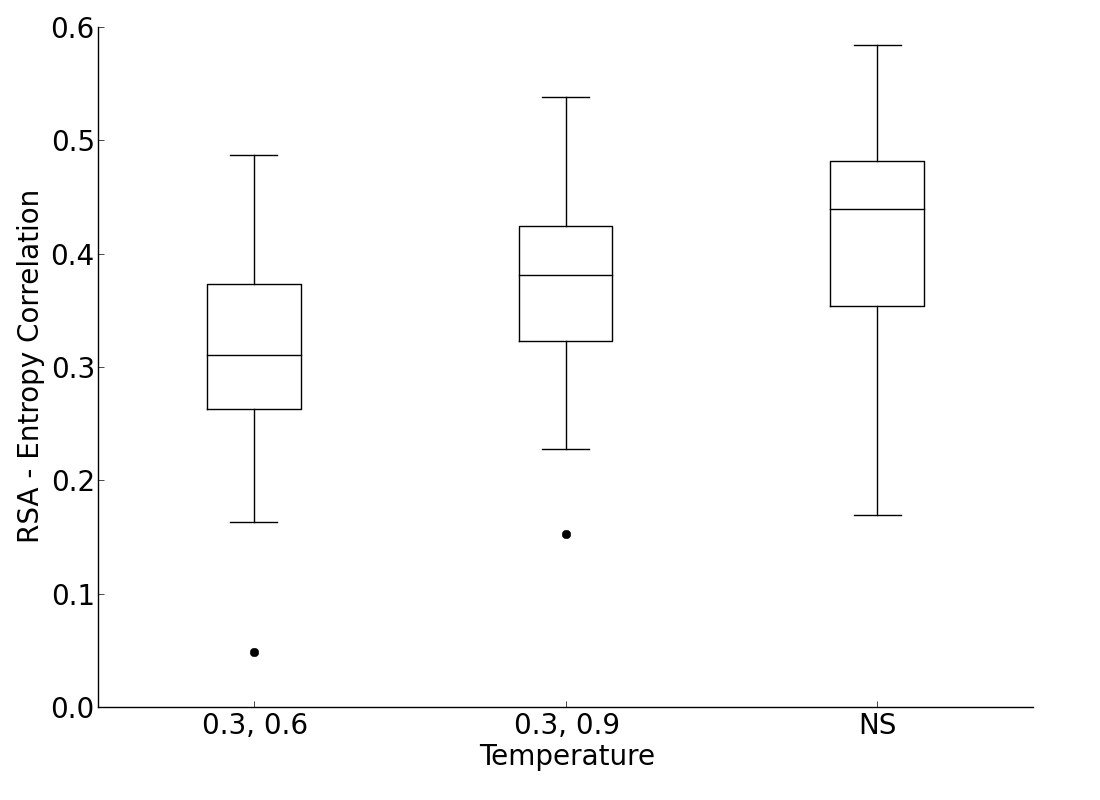
\includegraphics[width = 6in]{figures/Duncan_Mixed_Temp_Correlation_Plot.png}}
\caption{Correlation between RSA and Entropy between entropy at sites for 38 proteins. For each site we classified the site as buried if it had an RSA of than 0.05. All sites not classified as buried are classified as exposed. For sites that were buried, we used the frequencies from the T = 0.3 designed proteins. For the exposed sites we used either the entropy values from T = 0.6 or T = 0.9. By using the different temperature values for each type of site, the correlation between RSA and entropy of sites with the mixed entropy values were to that of the natural proteins.}
\label{Mixed_RSA_Entropy_Duncan}
\end{figure}

%Figure 25
\begin{figure}[H]
%\centering
\centerline{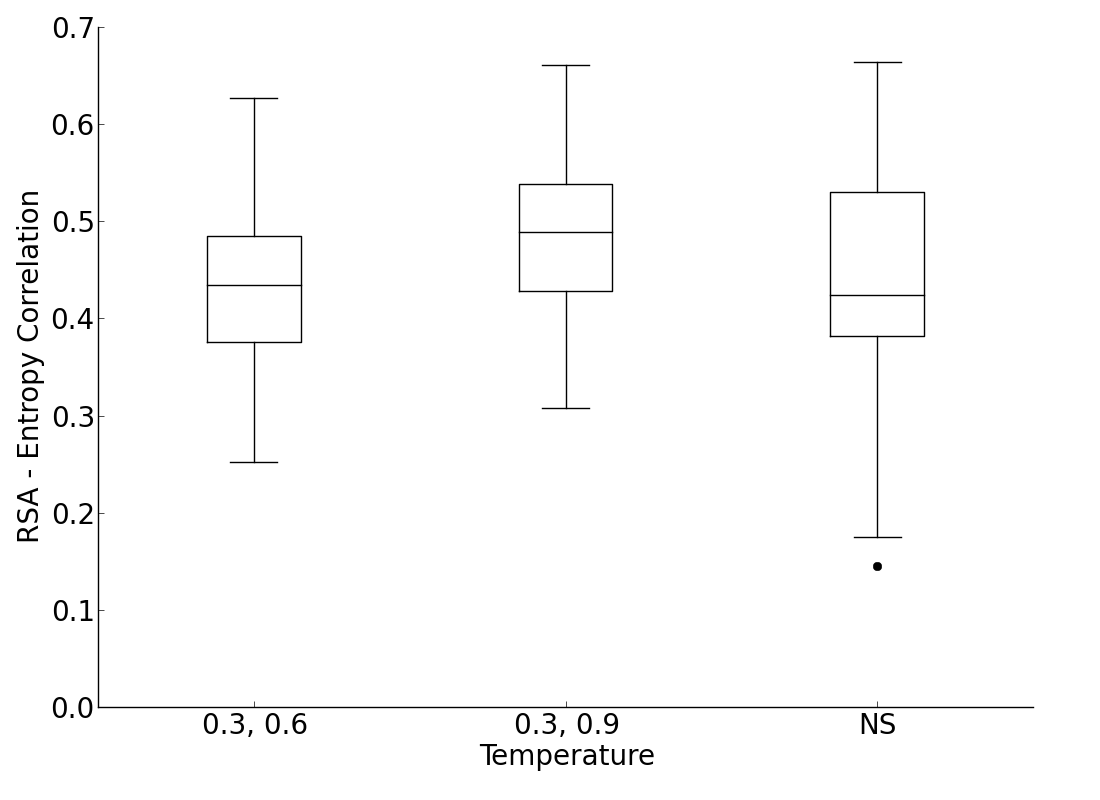
\includegraphics[width = 6in]{figures/Noah_Mixed_Temp_Correlation_Plot.png}}
\caption{Correlation between RSA and Entropy between entropy at sites for 40 protein domains. For each site we classified the site as buried if it had an RSA of than 0.05. All sites not classified as buried are classified as exposed. For sites that were buried, we used the frequencies from the T = 0.3 designed proteins. For the exposed sites we used either the entropy values from T = 0.6 or T = 0.9. By using the different temperature values for each type of site, the correlation between RSA and entropy of sites with the mixed entropy values were to that of the natural proteins.}
\label{Mixed_RSA_Entropy_Noah}
\end{figure}

%Figure 5
\begin{figure}[H]
\centering
\centerline{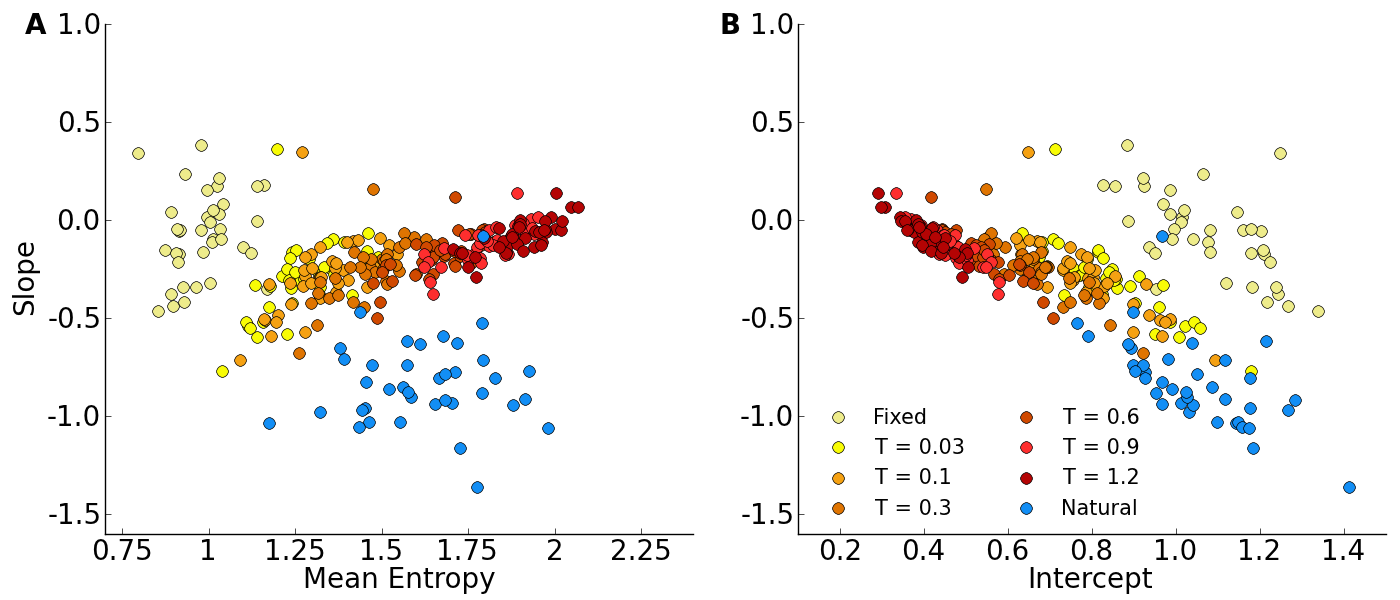
\includegraphics[width = 6in]{figures/Slope_Combination_Plot.png}}
\caption{Slopes calculated for 38 proteins. The slopes are calculated by fitting a linear function $\lambda=a\text{RSA}+b$ to these yeast proteins.  A) A plot of slope vs mean site entropy for 38 proteins. B) Intercepts vs Slopes for 38 proteins. Designed proteins have nonnegative slopes in contrast to the negative slope values found for natural proteins.  Natural proteins on average have a negative slope and a larger intercept when compared to designed proteins. Designed proteins on average have less negative slopes compared to natural proteins.}
\label{StructureFig3}
\end{figure}

%Figure 17
\begin{figure}[H]
\centering
\centerline{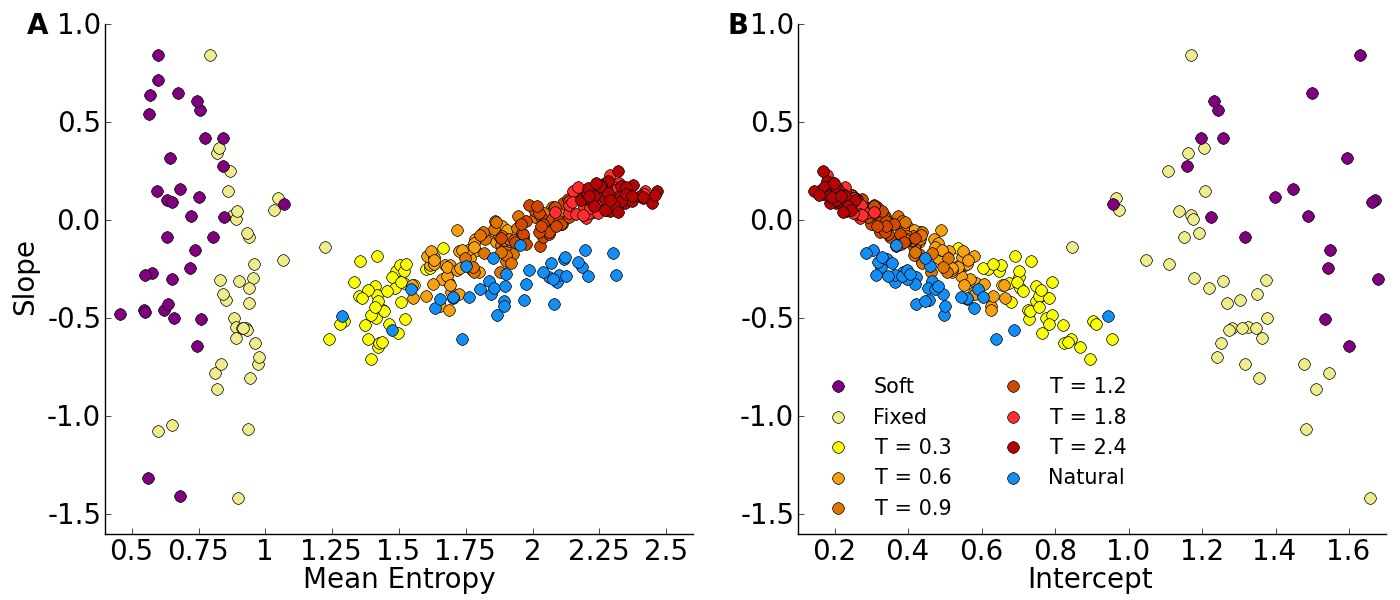
\includegraphics[width = 6in]{figures/Slope_Combination_Plot_Noah.png}}
\caption{Slopes calculated for 40 protein domains. The slopes are calculated by fitting a linear function $\lambda=a\text{RSA}+b$ to these yeast proteins.  A) A plot of slope vs mean site entropy for 40 protein domains. B) Intercepts vs Slopes for 40 protein domains. Designed proteins have nonnegative slopes in contrast to the negative slope values found for natural proteins.  Natural proteins on average have a negative slope and a larger intercept when compared to designed proteins.}
\label{NoahStructureFig3}
\end{figure}

\par Next we more closely examined how RSA affected the amino acid distributions at sites with both the natural and designed proteins. At each site within our protein alignments amino acids were ranked, k = 0,1,..., 20 corresponding to how frequent they were found at that site. Amino acid frequencies were found to be proportional to an exponential, $\exp (-\lambda k)$ as discovered in previous work \cite{Ramsey2011}. We used Maximum Likelihood Analysis (MLE) to fit the parameter $\lambda$ as a linear function of RSA in the form $$ \lambda = a \text{RSA} + b $$ $\lambda$ describes the shape of the amino acid distribution at site. A large $\lambda$ describes a distribution that is more skewed. A site with a large lambda means that often times there are only a few types amino acids that are observed at that site. The intercept, $b$, determines how much sequence variability is independent of RSA. A larger intercept means a larger $\lambda$, which leads to less variability. The slope, $a$, determines how much influence RSA has on $\lambda$. A slope of zero for a single protein means there is no difference between core and the surface amino acid distributions in that protein. Comparing the slopes and intercepts of the natural protein with the designed proteins allowed us understand how protein structure and site variability differ between the two different classes of proteins. 

\par Proteins designed with fixed backbones have intercept values that are most similar to natural proteins. Designed proteins with a flexible backbone have lower intercepts (Figure \ref{StructureFig3}B, \ref{NoahStructureFig3}B). In the natural proteins, most proteins had a negative slope. This means that there was less sequence variability at sites within the core when compared to sites on the surface.  On average the designed proteins had a larger slope than natural proteins (Figures \ref{StructureFig3}A, \ref{NoahStructureFig3}A) . In addition, as the temperature increased, the slope shifted and increased. This means that increasing temperature caused sites to exhibit more to be more site variability. The slope was positive because more mutations were allowed in the core protein. We conclude that proteins that are designed fail to accurately capture the restriction of acceptable amino acids within the protein core. 

\section{Discussion}
We designed a series of proteins from 38 natural yeast proteins. These designed proteins were used to create a series of alignments that we compared to natural alignments. These natural alignments were created using sequences that were homologous to the natural proteins used in the designed process.  We compared site variability as measured by entropy between the designed and natural proteins. Proteins that were designed with a backbone with intermediate flexibility exhibited site variability similar to sites within natural proteins. In addition, these proteins also had amino acid distributions at sites that are most similar in shape to sites within natural proteins. This suggests that not only do these proteins exhibit appropriate levels of site variability but they also more are accurate at using similar types of amino acids at those sites.  Lastly we used relative solvent accessibility to determine the effects of protein structure on site variability patterns in natural proteins. After measuring the effects of protein structure in natural proteins, we compared this effect to that of protein structure on designed proteins. 
\par Designed proteins appear to do a less accurate job at capturing the type of constraints that structure has on amino acid patterns at sites within natural proteins. According to our analysis, natural proteins had a much higher correlation between RSA and site variability. In natural proteins site variability is more strongly influenced by the site's position within the protein. In these proteins there is a much greater difference between the variability experienced by proteins on the surface of the protein and the variability experienced by sites with the proteins core. Designed proteins do not capture this difference.  Our results could help improve current software capabilities. The inability of Rosetta to accurately capture site variability differences between the core and the surface point to the need for improvements in determining scoring whether substitution should be made at a site. Improvements in the scoring functions of substitutions might lead to more accurately designed proteins in the future.
\bibliographystyle{plain} %"style
\bibliography{ProjectBib} %expected file "my refs.bib"

\section{Supplementary Figures}
\label{SupFigs}
\subsection{Additional Data Analyses}


\subsection{UCSF Dataset Analyses}
\label{UCSF}

%Figure 14
\begin{figure}[H]
\centering
\centerline{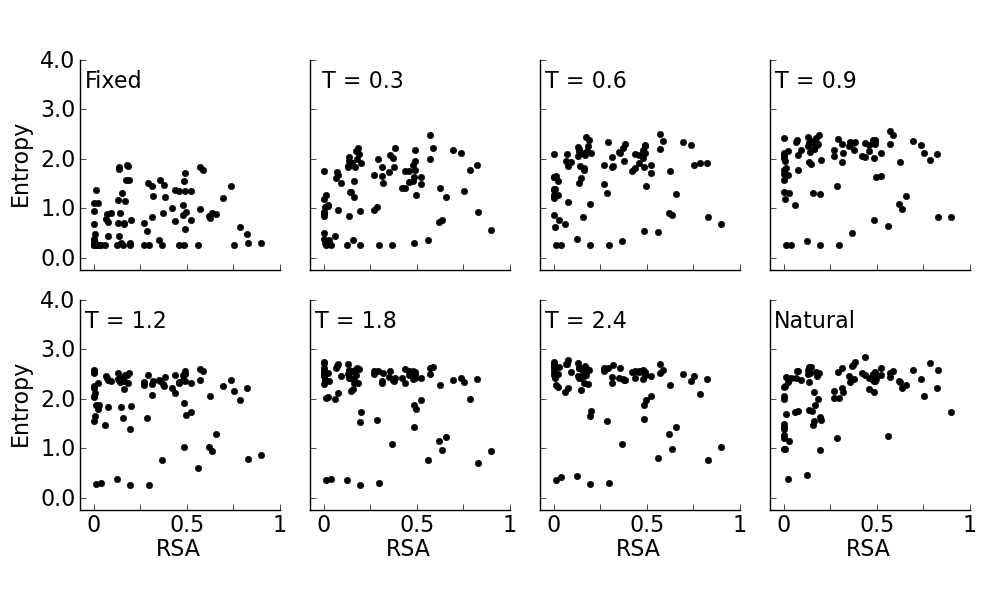
\includegraphics[width = 6.5in]{figures/RSA_vs_Entropy_2H3L_Combination_Plot_Noah.png}}
\caption{Entropy vs Relative Solvent Accessibility (RSA) for sites within the protein S - formylglutathione hydrolase (PDB: 2H3L, chain A). All RSA values are calculated from natural proteins. For most sites within the alignments created from the fixed backbone the entropy values are lower than they are in the natural proteins.}
\label{Entropy_Sites_Noah}
\end{figure}

%Figure 15
\begin{figure}[H]
\centerline{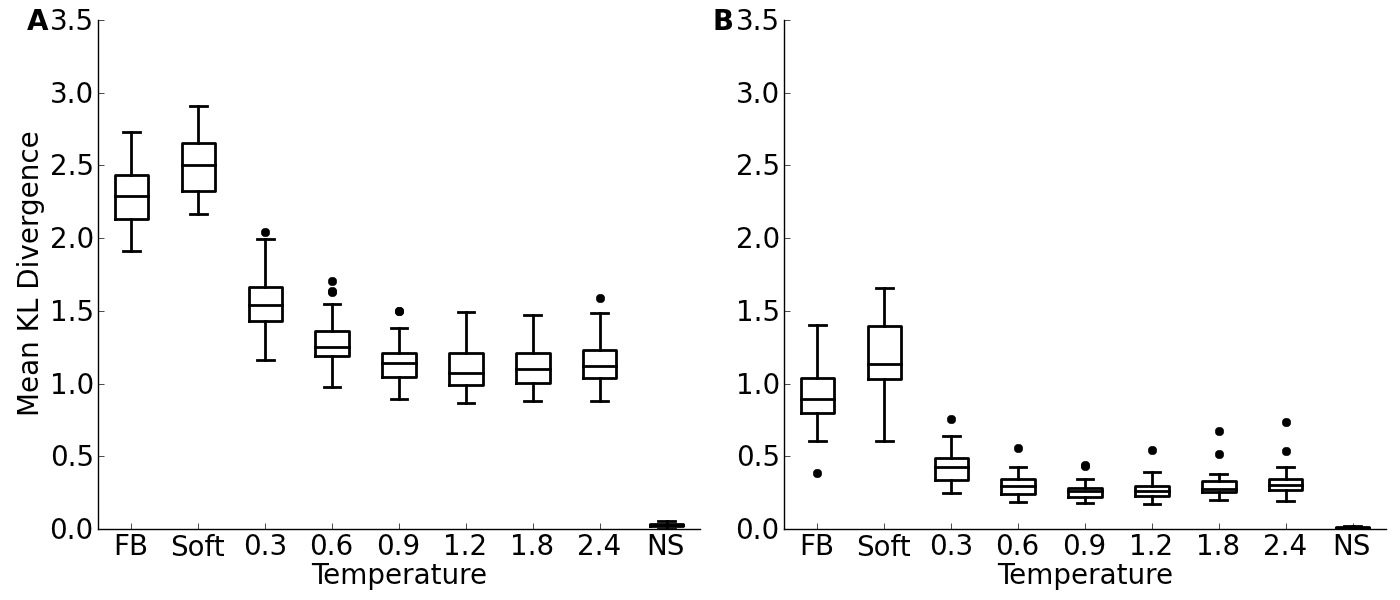
\includegraphics[width = 6in]{figures/Mean_KL_vs_Temp_Boxplot_Noah.png}}
\caption{Mean Kullback-Leibler (KL) Divergence Value vs Protein Design Temperature. Each boxplot corresponds to the mean KL Value for each of 500 designed proteins. Higher KL Divergence  equals a less similar distribution. The temperature refers to the temperature used when designing the proteins using BACKRUB and Mean KL Divergence stands for the mean Kullback-Liebler Divergence for each protein.  A) For these distributions, the amino acids are ordered by amino acid type, e.g., alanine, tyrosine. B) For these distributions the amino acids are ranked and ordered by their frequency with more frequent amino acids ranked first. Higher temperatures result in more backbone flexibility during design.}
\label{NoahAADisFig1}
\end{figure}

%Figure 16
\begin{figure}[H]
\centering
\centerline{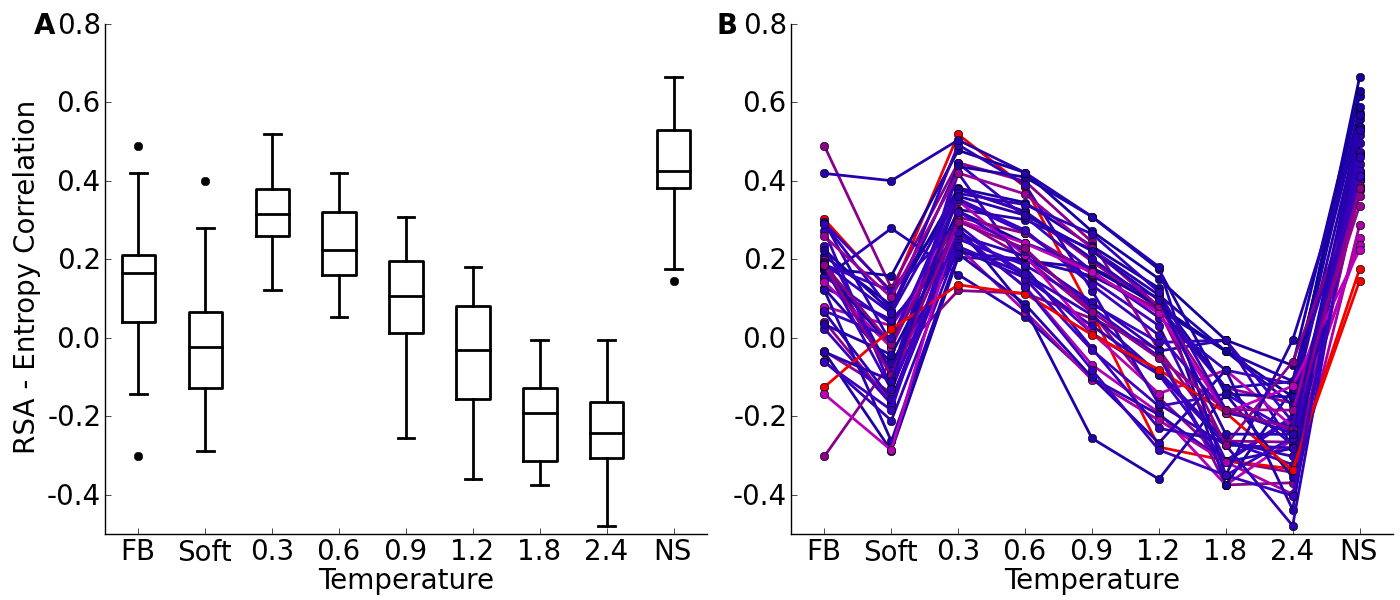
\includegraphics[width = 6in]{figures/Cor_Mean_Entropy_RSA_Combination_Plot_Noah.png}}
\caption{Correlation between Entropy and RSA for sites within proteins.  The temperatures represent alignments of designed proteins where an increased temperature relates to an increase level of backbone flexibility during the design process. A) Boxplots of the correlation between RSA and site entropy for various protein alignments. B) Lineplots of the correlation between RSA and site entropy for various protein alignments. The colors correspond to the value of the strength of the correlation between entropy and RSA at sites. }
\label{NoahStructureFig1}
\end{figure}

%Figure 21
\begin{figure}[H]
%\centering
\centerline{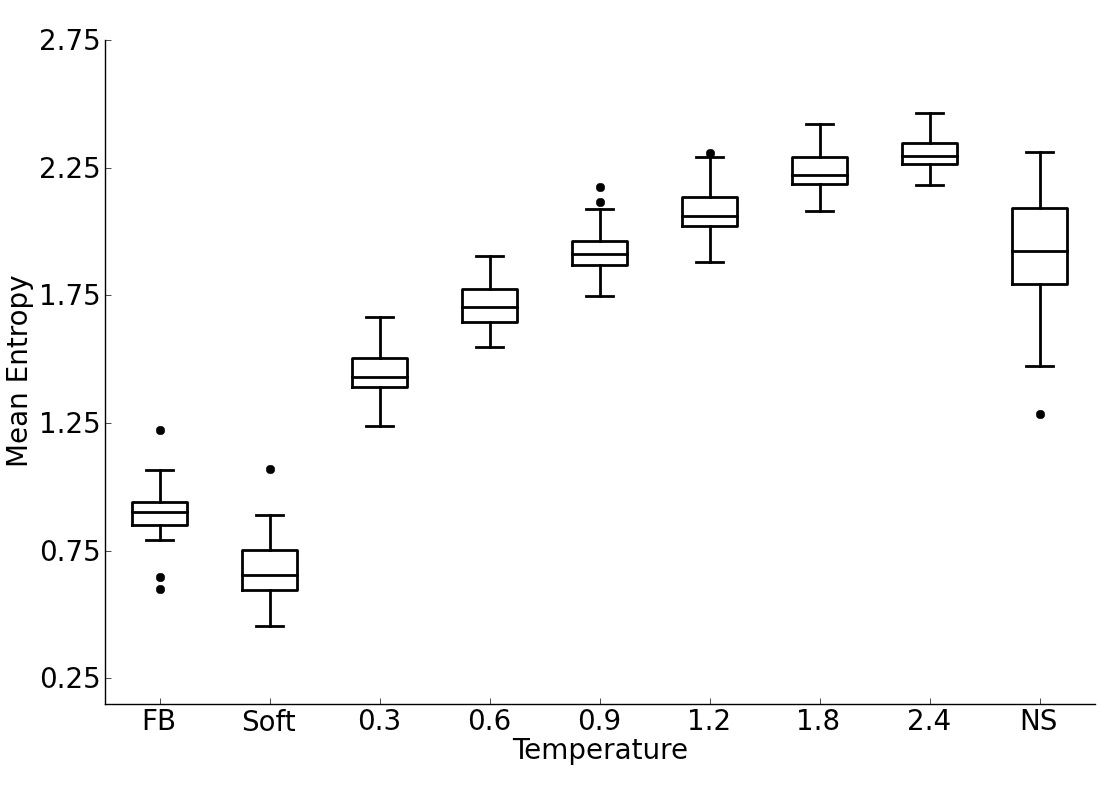
\includegraphics[width = 6in]{figures/Mean_Entropy_vs_Temp_Boxplot_Noah.png}}
\caption{Mean Entropy versus Temperature for sites within a series of designed proteins. The temperature refers to the temperature used during the designed process. Higher temperatures allowed for more backbone flexibility. FB and NS refer to the fixed backbone designed proteins and natural proteins respectively.  A site is categorized a buried site if it has an RSA of less than 0.05.}
\label{Mean_Entropy_Noah}
\end{figure}

%Figure 21
\begin{figure}[H]
%\centering
\centerline{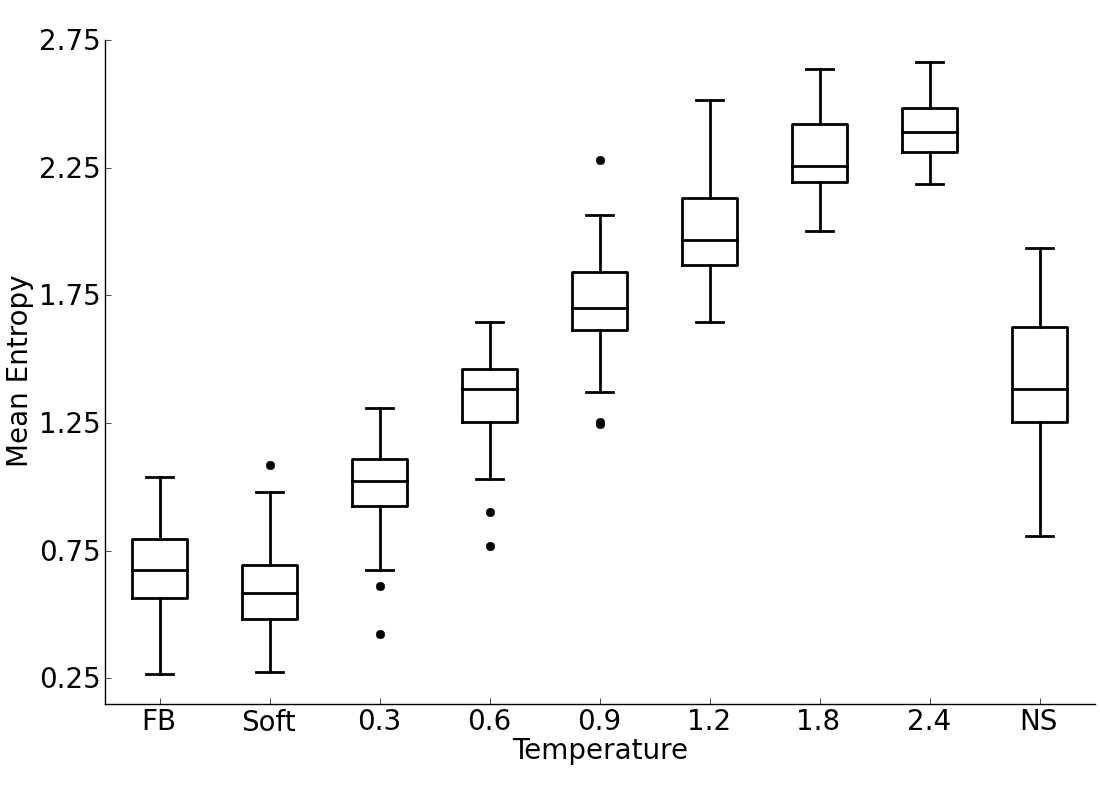
\includegraphics[width = 6in]{figures/Mean_Entropy_vs_Temp_Buried_Boxplot_Noah.png}}
\caption{Mean Entropy versus Temperature for buried sites within a series of designed proteins. The temperature refers to the temperature used during the designed process. Higher temperatures allowed for more backbone flexibility. FB and NS refer to the fixed backbone designed proteins and natural proteins respectively.  A site is categorized a buried site if it has an RSA of less than 0.05.}
\label{Buried_Entropy_Noah}
\end{figure}

%Figure 22
\begin{figure}[H]
%\centering
\centerline{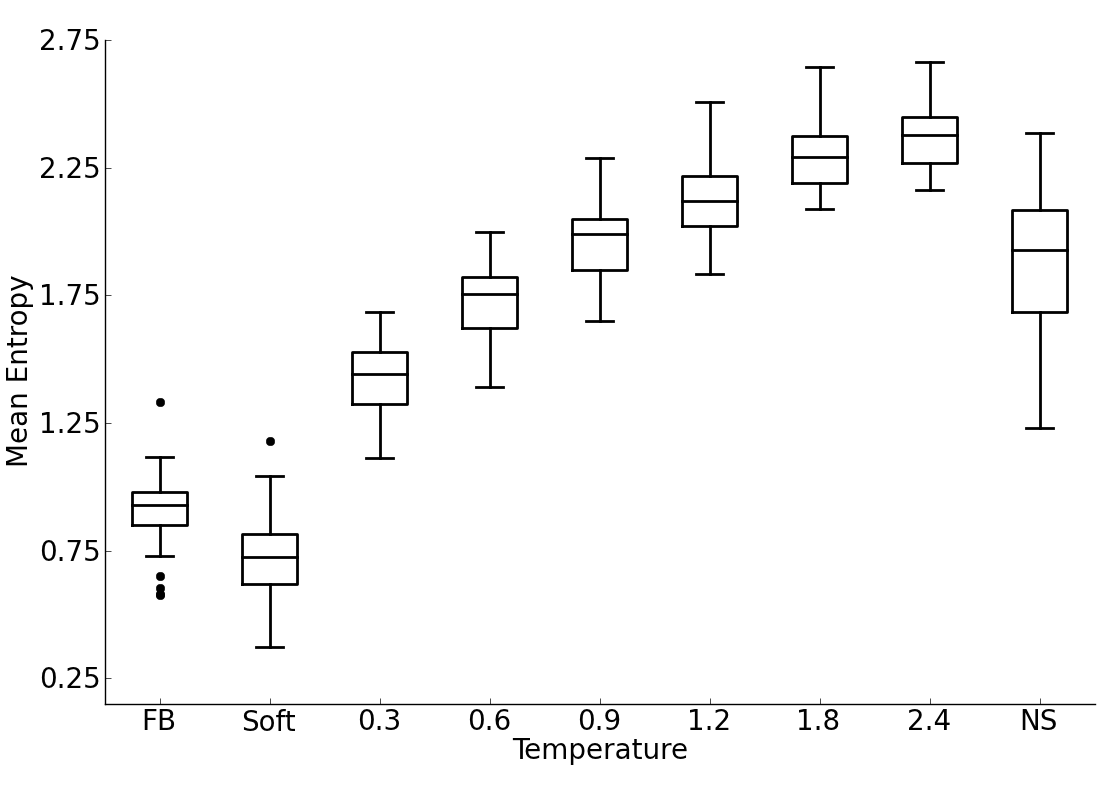
\includegraphics[width = 6in]{figures/Mean_Entropy_vs_Temp_Intermediate_Boxplot_Noah.png}}
\caption{Mean Entropy versus Temperature for partially buried sites within a series of designed proteins. The temperature refers to the temperature used during the designed process. Higher temperatures allowed for more backbone flexibility. A site is categorized as a partially buried site if it has a RSA of greater than or equal to 0.05 and less than or equal to 0.25. FB and NS refer to the fixed backbone designed proteins and natural proteins respectively.}
\label{Inter_Entropy_Noah}
\end{figure}

%Figure 23
\begin{figure}[H]
%\centering
\centerline{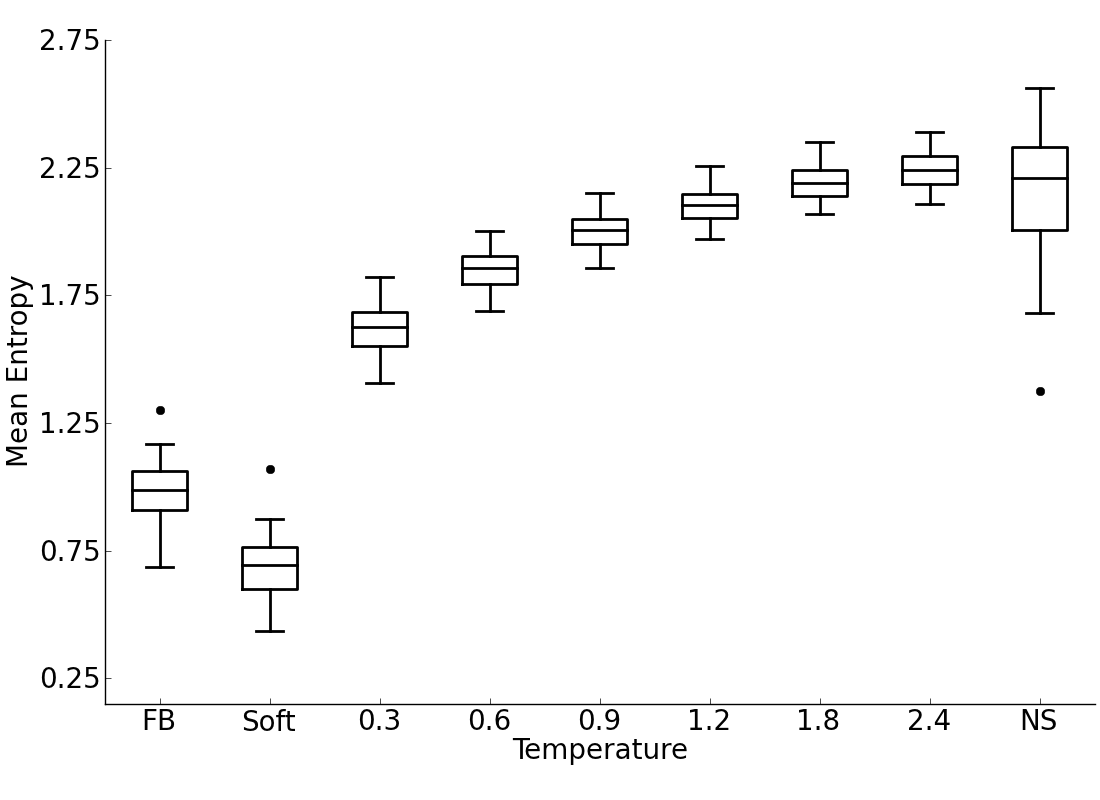
\includegraphics[width = 6in]{figures/Mean_Entropy_vs_Temp_Surface_Boxplot_Noah.png}}
\caption{Mean Entropy versus Temperature for exposed sites within series of 40 designed protein domains. The temperature refers to the temperature used during the designed process. Higher temperatures allowed for more backbone flexibility. A site is categorized as a surface site if it has a RSA of greater than 0.25. FB and NS refer to the fixed backbone designed proteins and natural proteins respectively.}
\label{Surface_Entropy_Noah}
\end{figure}

%Figure 24
\begin{figure}[H]
%\centering
\centerline{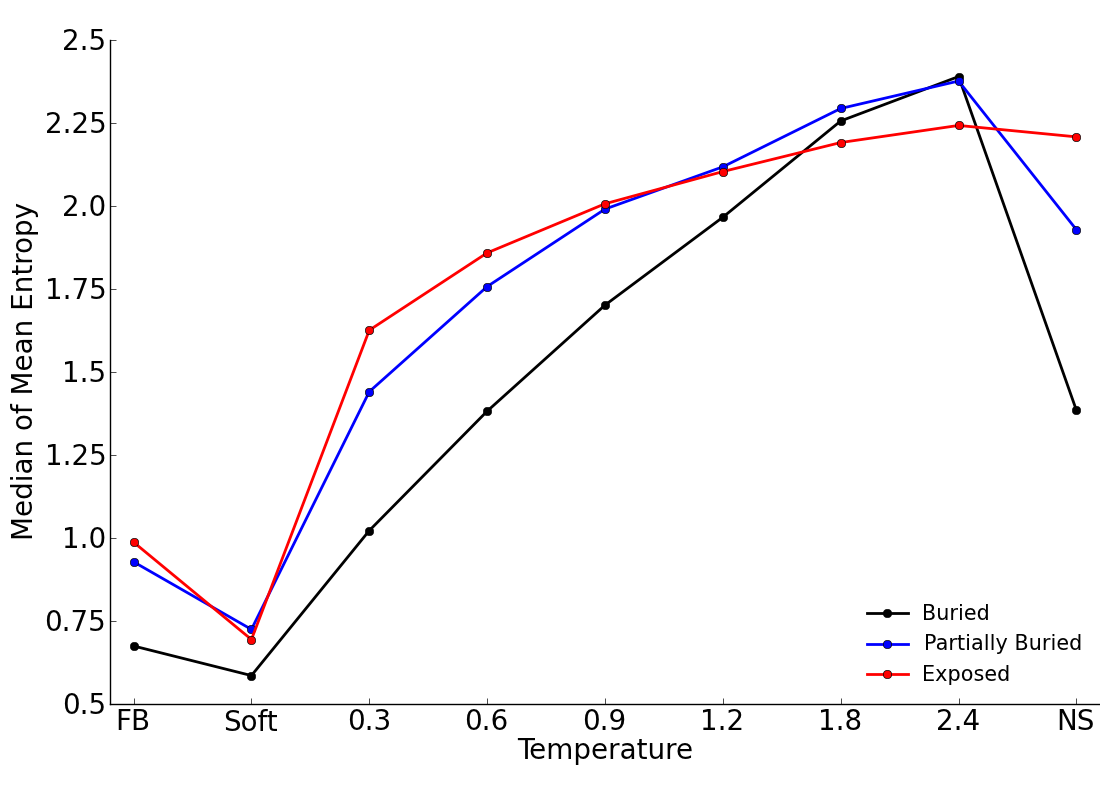
\includegraphics[width = 6in]{figures/Mean_Entropy_Position_Lineplot_Noah.png}}
\caption{Median of Mean Entropy versus Temperature sites within series of 40 designed protein domains.  Sites are classified as buried, partially buried, or exposed based on RSA magnitude. The temperature refers to the temperature used during the designed process. Higher temperatures allowed for more backbone flexibility. FB and NS refer to the fixed backbone designed proteins and natural proteins respectively.}
\label{Postion_Entropy_Noah}
\end{figure}

\end{document}